\section{Reock}\label{sec:reock}

Let $\mathrm{circ}(\Omega)$ denote the \textit{smallest bounding circle} (smallest bounding \textit{cap} on the sphere) of a region $\Omega$.  Then the \textit{Reock score} of $\Omega$ is 

$$\mathrm{Reock}(\Omega)= \frac{\mathrm{area}(\Omega)}{\mathrm{area}(\mathrm{circ}(\Omega))}.$$

In words, it is the ratio of the area of the region to the area of the smallest circle containing that region, and it is equal to one if and only if $\Omega$ is a circle.  We can observe that $\mathrm{CH}(\Omega)\geq \mathrm{Reock}(\Omega)$, since the convex hull of a region is never larger than the smallest bounding circle.  This relation holds with equality if and only if the convex hull of $\Omega$ is a circle.  

The similarity of this measure to the convex hull score suggest a similar tack for proving that no map projection can preserve the ordering of Reock scores, and indeed the structure of the proof is identical.  We proceed by demonstrating the following:

\begin{enumerate}
    \item Any map projection which preserves the ordering of convex hull scores must, in particular, preserve the maximizers in that ordering.  This means that such a projection must send caps on the sphere to circles in the plane.
    \item One projection which is convexity-preserving is the stereographic projection.
    \item Affine linear transformations of the plane which can be written as the composition of a scaling, a rotation, a reflection, and a translation preserve circles, i.e. a \textit{scaled isometry}.
    \item The set of scaled isometries is exactly the set of circle-preserving transformations of the plane.
    \item Any circle-preserving map projection must therefore be the composition of the stereographic projection and a scaled isometry.
    \item The stereographic projection does not preserve the ordering of Reock scores, and any scaled isometry \textit{does}.
    \item Therefore, there is no composition of the stereographic projection and a scaled isometry which together preserve the ordering of Reock scores.
\end{enumerate}


Since $\mathrm{Reock}(\Omega)=1$ if and only if $\Omega$ is a circle, we can observe that any candidate for a map projection which preserves the ordering of Reock scores must, at the very least, preserve the maximizeres in the ordering, meaning it sends caps on the sphere to circles in the plane.  The \textit{stereographic projection} is one such circle-preserving map projection, and we will show that the family of map projections which are circle-preserving are exactly those which can be written as the composition of the stereographic projection and a \textit{scaled isometry} of the plane.

\begin{definition}
The \textbf{stereograpic projection} from the sphere to the plane is defined by placing the plane tangent to the sphere at the south pole, and for any point $p$ on the sphere other than the north pole, $p$ is sent to the unique point $q$ in the plane which is on the line in 3-space passing through the north pole and $p$.

If $(x,y,z)$ is a point on the sphere, then the action of the stereographic projection is

$$(x,y,z)\mapsto \left(\frac{x}{1-z},\frac{y}{1-z}\right),$$

and its inverse, for $(u,v)$ in the plane:

$$(u,v)\mapsto \left( \frac{2u}{1+u^2+v^2},\frac{2v}{1+u^2+v^2}, \frac{u^2+v^2-1}{1+u^2+v^2}   \right).$$


\end{definition}




What is somewhat surprising is that this projection sends every cap on the sphere which doesn't pass through the north pole to a circle in the plane.  There are several proofs of this fact, and we present a rather straightforward algebraic one here.

\begin{lemma}
The stereographic projection sends every cap which does not pass through the north pole to a circle in the plane.
\end{lemma}
\begin{proof}

We proceed algebraically.  Since a cap on the sphere can be identified by the plane in $\R^3$ which intersects the sphere along its boundary, we can parametrize such a cap by writing the equation for its corresponding plane, $ax+by+cz=d$, restricting $(x,y,z)$ to be points on the sphere.  The image in the plane of this cap is some set of $(u,v)$ points, and we can explicitly write this by substituting in for $x$, $y$, and $z$ the corresponding values for the inverse stereographic projection.  We write $\mathcal{W}=u^2+v^2$ for the ease of presentation. 

\begin{align*}
    d&=ax+by+cz\\
    d&=a\left(\frac{2u}{1+u^2+v^2}\right)+b\left(\frac{2v}{1+u^2+v^2}\right)+c\left(\frac{u^2+v^2-1}{1+u^2+v^2}\right), \text{ by substitution}\\
    d&=a\left(\frac{2u}{1+\mathcal{W}}\right)+b\left(\frac{2v}{1+\mathcal{W}}\right)+c\left(\frac{\mathcal{W}-1}{1+\mathcal{W}}\right), \text{ by change-of-variable }\mathcal{W}=u^2+v^2\\
    d\left(1+\mathcal{W}\right)&=2au+2bv+c\left(\mathcal{W}-1\right), \text{ multiplying through by }1+\mathcal{W}\\
    0 &= (c-d)\mathcal{W} + 2au +2bv - c - d,\text{ by rearrangement}\\
    0 &= (c-d)(u^2+v^2)+2au+2bv - c - d,\text{ by change-of-variable } \mathcal{W}=u^2+v^2
\end{align*}

This last line is the equation of a circle in the plane if $c\neq d$ and a line otherwise.  Since $c=d$ if and only if the point $(x,y,z)=(0,0,1)$ (i.e. the north pole) is on the plane, and we assumed that this is not the case, we have shown that the image under the stereographic projection of every cap which does not pass through the north pole is a circle in the plane.

\end{proof}


We now have in-hand a circle-preserving map projection, and we now turn to demonstrating that the stereographic projection is essentially the unique map projection with this property.  We can observe that if we perform stereographic projection and compose it with a transformation of the plane which sends every circle to a circle, then this composition is a circle-preserving map projection.  The next lemma demonstrates that the class of transformations of the plane which preserve circles is actually quite narrow.

\begin{lemma}
If $T$ is a transformation of the plane which sends every circle in the plane to another circle, then $T$ must be a linear transformation which is the composition of a scaling, a rotation, a reflection, and a translation, i.e. a scaled isometry.
\end{lemma}
\begin{proof}

We first argue that if we restrict our attention to \textit{linear} transformations, the scaled isometries are the only transformations which preserve circles.  

If $T$ is a scaled isometry with scaling factor $\alpha$, then, by definition, for any points $x$ and $y$, the distance between $T(x)$ and $T(y)$ is $\alpha$ times the distance between $x$ and $y$.  Therefore, if we choose a circle $Y$ of radius $r$ and let $x$ be the center, then for any $y\in Y$, $d(T(x),T(y)) = \alpha r$, so $T(Y)$ is a circle of radius $r$.

Next, if $T$ is a linear transformation which is \textit{not} a scaled isometry, then we can find three points $x$, $y$, and $z$ such that $d(T(x),T(y)) = \alpha d(x,y)$ but $d(T(x),T(z)) \neq \alpha d(x,z)$.  Furthermore, since linear transformations preserve ratios of lengths of collinear segments, and we have two segments whose ratios of lengths are not preserved, these three points cannot be collinear, so we can consider the circle centered at $x$ and passing through $y$ and $z$.  But, since the ratio of lengths isn't preserved, $T$ distorts this circle, so $T$ is not circle-preserving.

We next need to rule out the existence of a non-linear transformation $T$ which is circle preserving.  We proceed by contradiction.  Suppose that $T$ is non-linear and circle-preserving.  Then, since $T$ is non-linear, there is some line $\ell$ such that the image $T(\ell)$ is not a line, so we can find three points $x$, $y$, and $z$ which are collinear, but $T(x)$, $T(y)$, and $T(z)$ are not.  Therefore, we can find a unique circle $C_T$ passing through $T(x)$, $T(y)$, and $T(z)$.  Let $T(a)$ be some other point on this circle, and we consider the preimage of this point, $a$.  If $a$ is not on the line $\ell$, then we can construct two circles, one passing through $a$, $x$, and $y$ and one passing through $a$, $y$, and $z$.  These two circles intersect at only two points, $a$ and $y$, but both of these circles are sent to $C_T$ by $T$, which is impossible if $T$ is injective.  Therefore, $a$ must lie on the line $\ell$.

By repeating this argument, any point on the circle $C_T$ must be the image of some point on $\ell$.  By continuity, we can see that every point on $\ell$ is sent to a point on $C_T$, but the homeomorphic image of a line cannot be a circle, so such a non-linear $T$ cannot exist.

Thus, a transformation of the plane is circle-preserving if and only if it is a scaled isometry.


\end{proof}

We can put these two pieces together to prove the main tool of this section -- that any map projection from the sphere to the plane which preserves circles is the composition of the stereographic projection and a scaled isometry.

\begin{lemma}
The map projections from the sphere to the plane which send every cap to a circle are exactly those which can be written as the composition of the stereographic projection followed by a scaled isometry of the plane.
\end{lemma}
\begin{proof}
Let $\varphi$ and $\psi$ be two map projections which preserve circles, 
and without loss of generality let $\varphi$ be the standard stereographic projection.  
Then the composition $T=\psi\circ\varphi^{-1}$ is a transformation of the plane which preserves circles, so by the previous lemma, $T$ is a scaled isometry.  Then, we can write 
$\psi= T^{-1}\varphi$, which is the composition of the stereographic projection and a scaled isometry.
\end{proof}

As in the previous section, we can construct an example of two regions whose Reock scores are permuted by the stereographic projection.  In fact, we can use \textit{exactly} the same pair of regions as in the convex hull settings, as is made clear by the following lemma.



\begin{lemma}
Let $\varphi$ be the stereographic projection and $C_\theta$ be a spherical cap centered at the south pole parametrized by the angle $\theta <\pi/4$ formed between the central axis of the sphere and the line of projection passing through the north pole and the boundary of the cap (Figure~\ref{fig:stereocap}). Then $\phi(C_\theta)$ is a disk in the plane, centered at the origin, and has radius $2\tan\theta$
\end{lemma}
\begin{figure}
    \centering
    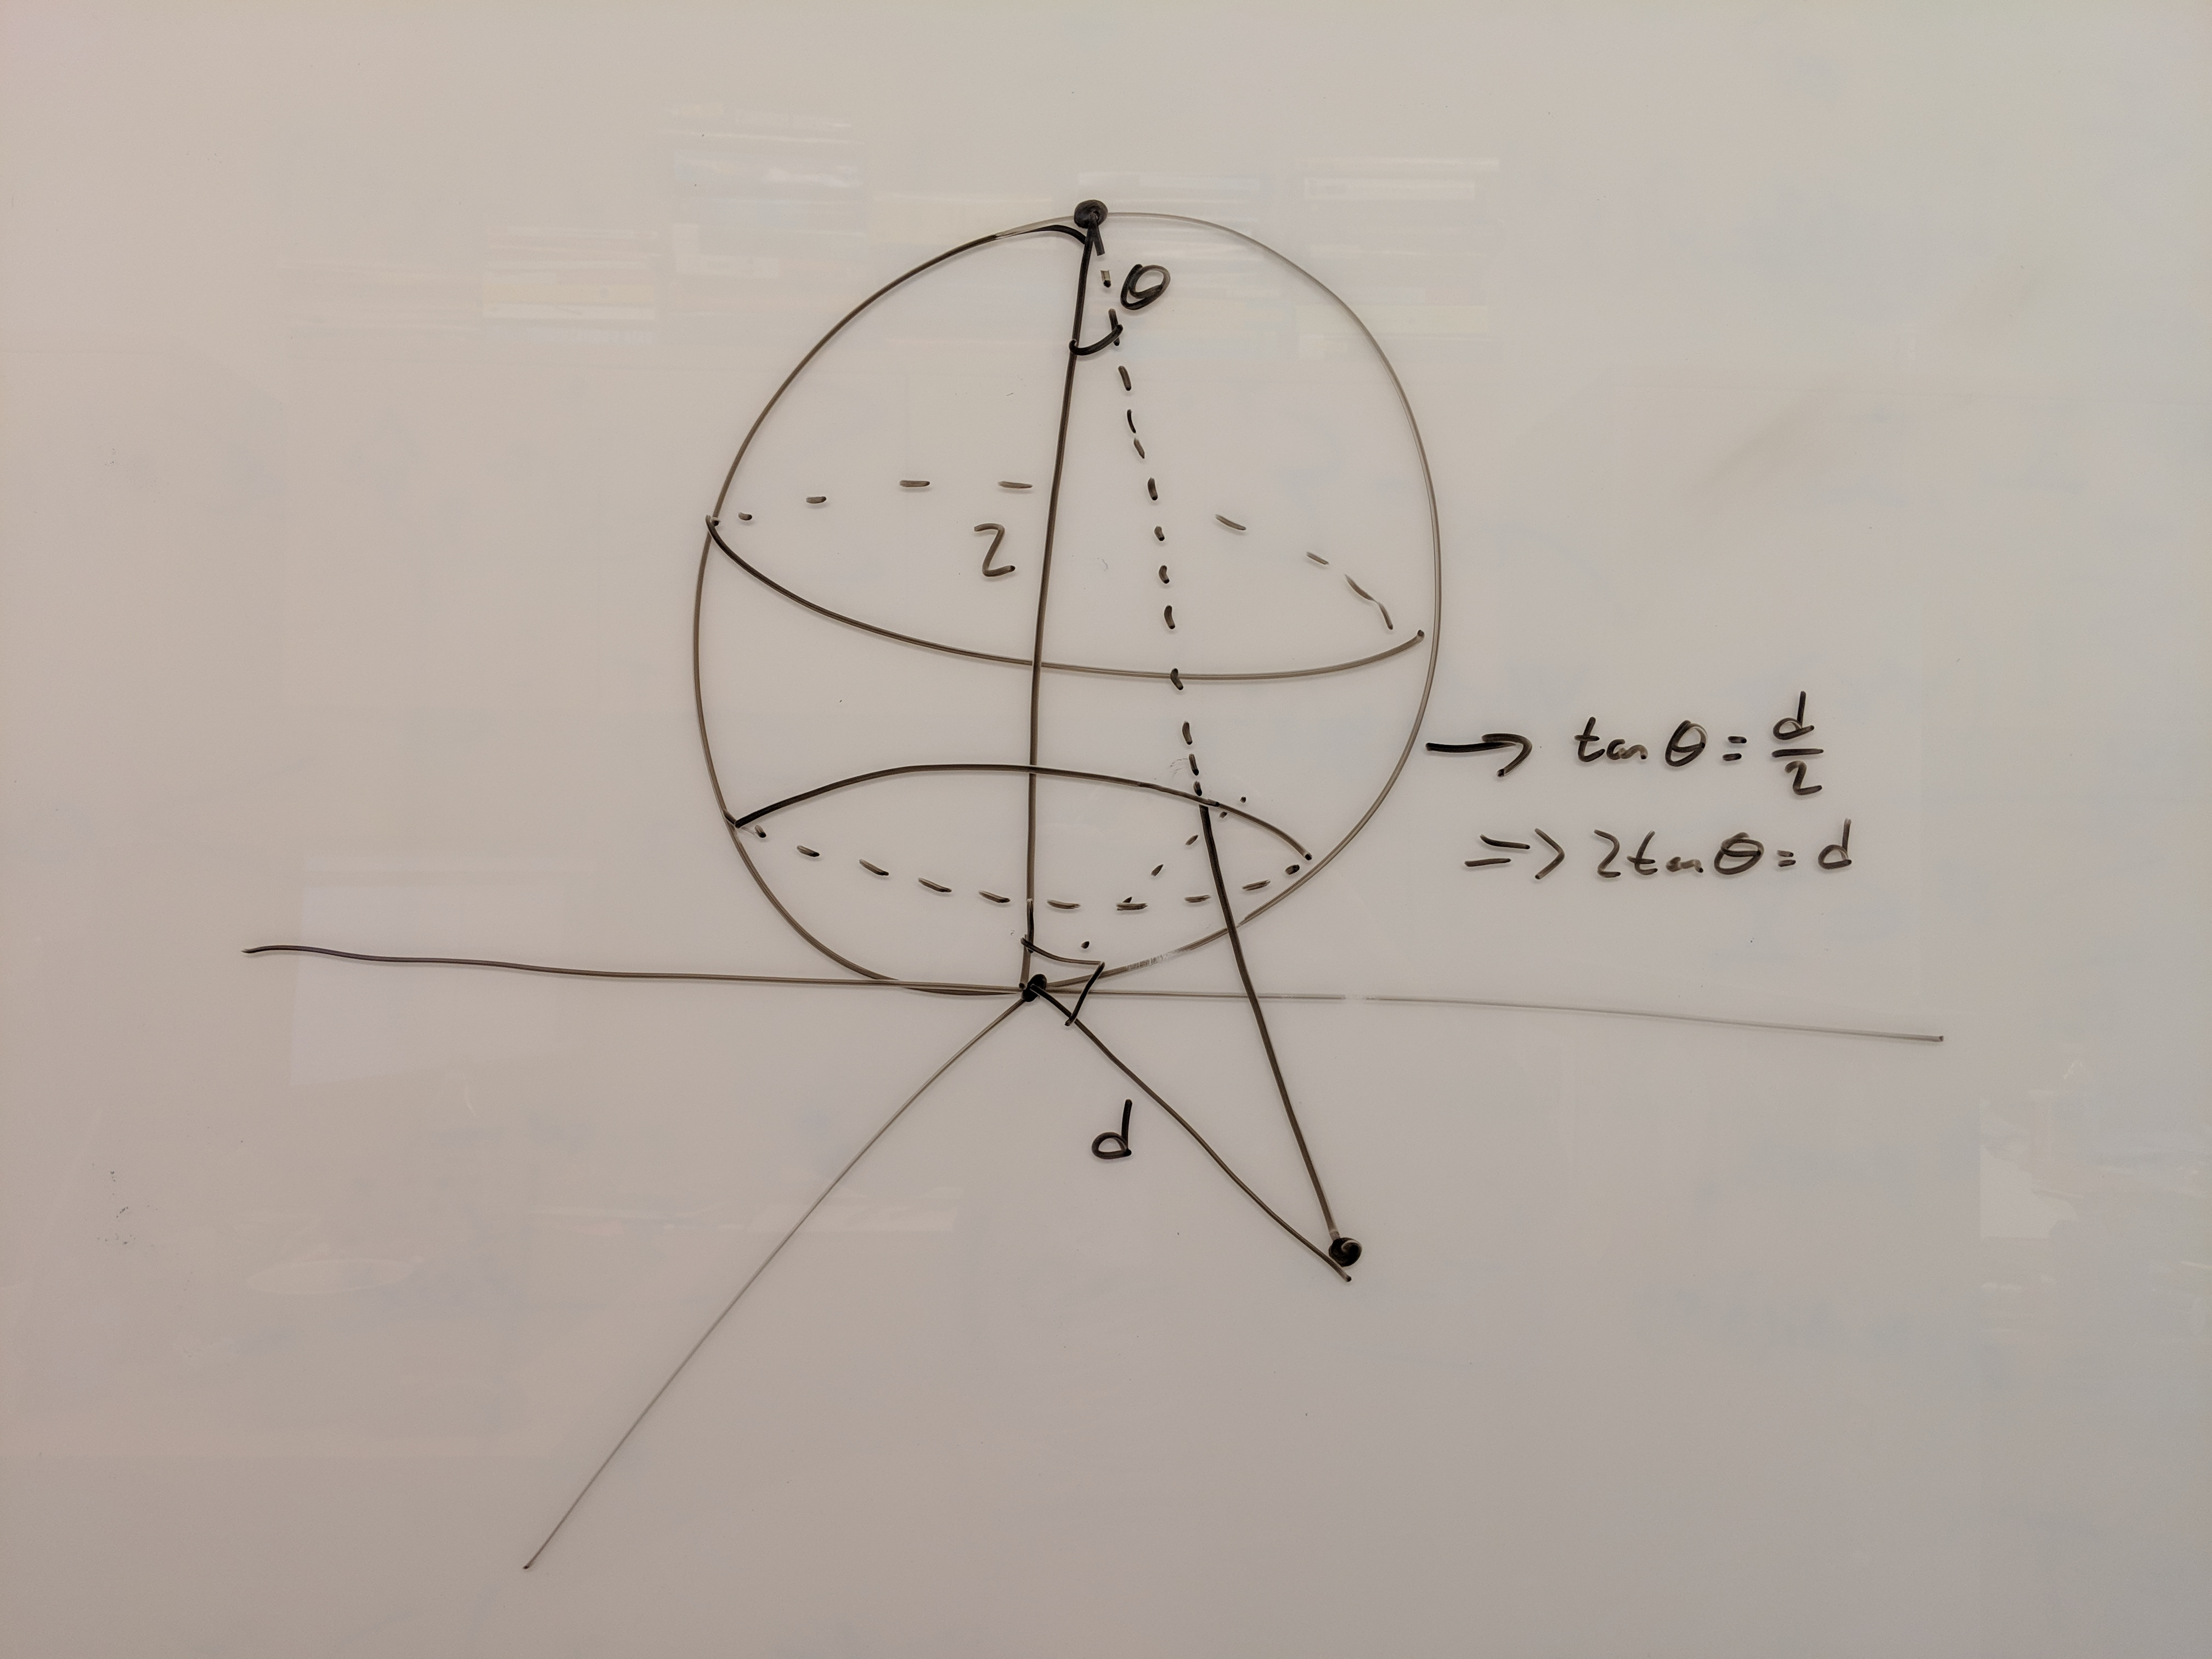
\includegraphics[width=.8\textwidth]{figs/stereo_cap.jpg}\\
    \caption{ The image of a cap with angle $\theta$ between the polar axis and the line of projection is a circle of radius $2\tan\theta$.  }
    \label{fig:stereocap}
\end{figure}
\begin{proof}


Since $\varphi$ projects from the north pole of the sphere and the sphere's south pole is mapped to the origin in the plane, the image of $C_\theta$ is totally radially symmetric about the origin, and is therefore a circle.  To see that its radius is $2\tan(\theta)$, place the south pole of the sphere tangent to the plane at the origin. By construction, for any point $p$ on the boundary of $C_\theta$, there is a unique line passing through the north pole of the sphere, $p$, and the point $\varphi(p)$ on the boundary of the disk in the plane.  By definition, this line meets the central axis of the sphere at an angle of $\theta$, and the central axis of the sphere meets the plane orthogonally, so the center of the sphere, the origin, and the point $\varphi(p)$ form a right triangle with angle $\theta$.  Since we know that the distance between the north pole of the sphere and the origin is 2, we can write the distance between the origin and $\varphi(p)$ as $2\tan(\theta)$.

\end{proof}

Since the properties of the stereographic projection near the origin is structurally so similar to that of the gnomonic projection, the exact same pair of regions serves as the counterexample in this setting as well.  When we examine the Reock scores of the projected regions in the plane, the factors of two cancel out.



We now have a concrete example of the stereographic projection permuting scores, by Lemma~\ref{lem:noafflin} in the previous section, since scaled isometries are a special kind of affine linear transformations, they too preserve ratios of areas and therefore Reock scores.  We can conclude this section by summarizing the proof of the main result.

\begin{theorem}
There is no map projetion from the sphere to the plane which preserves the ordering of Reock scores.
\end{theorem}
\begin{proof}
Since such a projection must send caps on the sphere to circles in the plane, it must be the composition of the stereographic projection with a scaled isometry of the plane.  Since scaled isometries preserve Reock scores and therefore their ordering, a Reock score order-preserving projection from the sphere to the plane cannot exist if the stereographic projection does not preserve the ordering.  By the constructed counterexample, it does not, and therefore there is no such Reock score ordering map projection.
\end{proof}
